\section*{Лекція 14: Об’єкти та класи}
\subsection{Вступ до ООП} 

\begin{frame}
\frametitle{ООП та класи}
ООП - об'єктно орієнтоване програмування. В програмах ми оперуємо об'єктами даних. Об'єкт даних - екземпляр класу.

\begin{figure}
  \begin{center}
    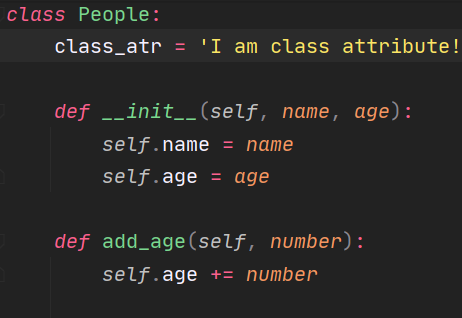
\includegraphics[width=0.4\textwidth,height=0.4\textheight]{pictures/class.png}
  \caption{Приклад класу в Python}
\label{function}
  \end{center}
\end{figure}

\end{frame}

\begin{frame}
\frametitle{Особливості ООП}
\begin{itemize}
  \item Класи та об'єкти класів.
  \item Клас містить властивості та методи.
  \item Інкапсуляція. Дані та методи класу можна приховувати.
  \item Успадкування. Дочірні класи можуть розширювати функціональність базових.
  \item Поліморфізм. Можливість через единий інтерфейс працювати з об'єктами різних класів.
\end{itemize}

\end{frame}

\begin{frame}
\frametitle{Функція isinstance}

Функція \texttt{isinstance(obj, type)} перевіряє чи належить об'єкт \texttt{obj} до типу даних \texttt{type} і повертає \texttt{True} або \texttt{False}. Замість \texttt{type} можна використовувати кортеж із декількох типів даних.

Тип \texttt{bool} успадковується від типу \texttt{int}, тому ця функція показує, що значення \texttt{True} або \texttt{False} належать до типу \texttt{int}.

Перевірку типу даних також можна робити за допомогою функції \texttt{type}:

\texttt{type(a) == int} або \texttt{type(a) in (int, float)}  

\end{frame}

\subsection{Класи та їх атрибути} 
\begin{frame}
\frametitle{Визначення класу}

Name - назва класу, attr\_1 та attr\_2 - атрибути класу. 

\texttt{class Name:}

\texttt{~~~~attr\_1}

\texttt{~~~~attr\_2}

 Фактично клас створює простір імен з назвою Name. Атрибути класу можна знайти в словнику \texttt{Name.\_\_dict\_\_}. Створення екземпляра класу \texttt{a = Name()}.
 
 \texttt{Name.\_\_doc\_\_} - містить рядок з описом класу.
\end{frame}

\begin{frame}
\frametitle{Робота з атрибутами класів}

\begin{itemize}
  \item <1-> \texttt{Name.attr = val} (\texttt{setattr(Name, 'attr', val)}) - додає до класу \texttt{Name} атрибут \texttt{attr} зі значенням \texttt{val}.
  \item <2-> \texttt{obj.attr = val} - додає до екземпляру класу \texttt{obj} атрибут \texttt{attr} зі значенням \texttt{val}.
  \item <3-> \texttt{Name.attr} (\texttt{getattr(Name, 'attr', val)}) - читає атрибут \texttt{attr} класу \texttt{Name}, якщо такий атрибут відсутній видає помилку (\texttt{val}).
  \end{itemize}

\end{frame}

\begin{frame}
\frametitle{Робота з атрибутами класів}

\begin{itemize}
  \item <1-> \texttt{hasattr(Name, 'attr')} - перевіряє чи є в класі \texttt{Name} атрибут \texttt{attr}.
  \item <2->\texttt{del Name.attr} (\texttt{delattr(Name, 'attr')} ) - видаляє з класу \texttt{Name} атрибут \texttt{attr}, якщо атрибут відсутній видає помилку.
 \end{itemize}
Для об'єкту класа спочатку атрибут шукається в поточному просторі імен, а потім в просторі імен класу.
\end{frame}

\subsection{Методи класів} 
\begin{frame}
\frametitle{Виклик методу класа}

Методи - це якісь дії.

Параметр \texttt{self} дозволяє дізнатися, з яким із екземплярів класу працює метод.

Викликати метод \texttt{set} для екземпляра \texttt{obj} класа \texttt{Name} можна так:

 \begin{center}
 \texttt{Name.set(obj)} або \texttt{obj.set()}.
 \end{center} 

\end{frame}

\begin{frame}
\frametitle{Ініціалізатор та фіналізатор}

Магічні методи розпочинаються та закінчуються двома символами підкреслення.

\texttt{\_\_init\_\_(self)} - викликається відразу після створення класу.

\texttt{\_\_del\_\_(self)} (фіналізатор) - викликається безпосередньо перед видаленням класу. 

У Python є збирач сміття, який видаляє об'єкти щойно вони стають непотрібними.

\end{frame}

\begin{frame}
\frametitle{Магічний метод \_\_new\_\_}

\texttt{\_\_new\_\_} - викликається перед створенням класу, поваертає адресу нового створеного об'єкту. 

\vspace{0.5cm}

\texttt{def \_\_new\_\_(cls, *args, **kwargs):} 

\texttt{~~~~якісь команди} 

\texttt{~~~~return super().\_\_new\_\_(cls)} 

\vspace{0.5cm}

\texttt{cls} посилається на поточний екземпляр класу. \texttt{super()} - посилається на базовий клас.

\end{frame}

\begin{frame}
\frametitle{Паттерн Singleton}
Екземпляр класу в кожний момент часу повинен бути лише один. Приклад для класу Name:

\texttt{\_\_instance = None}
 
\texttt{def \_\_new\_\_(cls, *args, **kwargs):} 

\texttt{~~~~if cls.\_\_instance is None:} 

\texttt{~~~~~~~~cls.\_\_instance = super().\_\_new\_\_(cls)} 

\texttt{~~~~return cls.\_\_instance} 

\texttt{def \_\_del\_\_(self):} 

\texttt{~~~~Name.\_\_instance = None}

\end{frame}

\begin{frame}
\frametitle{Методи класу}

Метод класу об'явлюється за допомогою декоратора \texttt{@classmethod}, як обов'язковий аргумент приймає посилання на поточний екземпляр класу \texttt{cls}. Приклад:
\vspace{0.3cm}

\texttt{@classmethod}

\texttt{def method(cls, args):}

\texttt{~~~~some operations}
\vspace{0.3cm}
Метод класу працює з атрибутами класу, але не може звертатися до атрибутів екземпляра класу. Виклик методу класу: \texttt{Name.method(arg)}
\end{frame}

\begin{frame}
\frametitle{Статичні методи}
Статичні методи не мають доступу ні до атрибутів класу, ні до атрибутів його екземпляра. Вони об'явлюються за допомогою декоратора \texttt{@staticmethod}. Приклад:

\vspace{0.3cm}
\texttt{@staticmethod}

\texttt{def method(cls, args):}

\texttt{~~~~some operations}
\vspace{0.3cm}

Використовується для створення незалежних сервісних функцій всередині класу.  
\end{frame}




\subsection{Успадкування}
 
\begin{frame}
\frametitle{Що таке успадкування?}
\begin{figure}
\begin{center}
 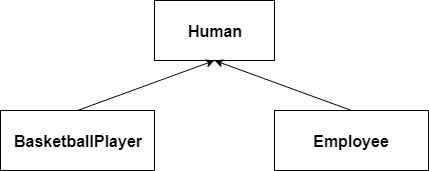
\includegraphics[width=0.4\textwidth]{pictures/inheritance.jpg}
\caption{Успадкування}
\label{inheritance} 
\end{center}
\end{figure}

На малюнку \texttt{Human} - базовий або батьківський клас, а \texttt{BasketballPlaeyr} та \texttt{Employee} - підкласи або дочірні класи.

\end{frame}

\begin{frame}
\frametitle{Приклад батьківського класу}
Відкриті атрибути батьківського класу є доступними із класів-спадкоємців.

\begin{figure}
\begin{center}
 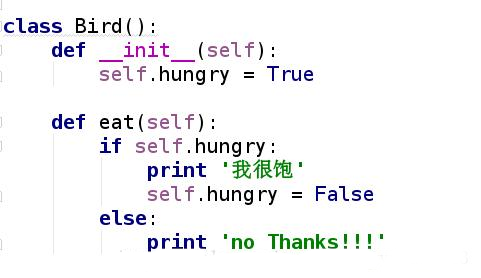
\includegraphics[width=0.4\textwidth]{pictures/class-bird.png}
\caption{Успадкування}
\label{inheritance} 
\end{center}
\end{figure}

\end{frame}

\begin{frame}
\frametitle{Приклад класів спадкоємців}

Метод спочатку шукається в поточному класі, а потім (якщо його не знайдено) - в батьківському класі. 

\begin{figure}
\begin{center}
 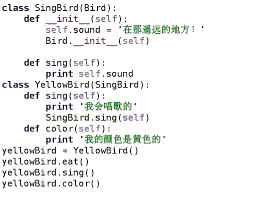
\includegraphics[width=0.4\textwidth]{pictures/class-signbird.png}
\caption{Успадкування}
\label{inheritance} 
\end{center}
\end{figure}

\end{frame}

\begin{frame}
\frametitle{Делегування}
\texttt{class Name:}

\texttt{~~~~def \_\_init\_\_(self):}

\texttt{~~~~~~~~pass}

\texttt{class Subname(Name):}

\texttt{~~~~def \_\_init\_\_(self):}

\texttt{~~~~~~~~super().\_\_init\_\_()}
 
Функція \texttt{super()} посилається на об'єкт базового класу. Виклик методів базового класу через функцію \texttt{super()}  називається \underline{делегування}.
\end{frame}
